\section{Datasets}

\begin{table*}[!htp]
\tiny
\caption{Twitter datasets studied in this chapter.} % title of Table
\vspace{0.5em}
\centering % used for centering table
\begin{tabular}{| p{0.3cm} | p{1.2cm} | p{1.4cm} | p{1.6cm} | p{0.8cm} | p{1.1cm} | p{0.8cm} | p{1.4cm} | p{4.2cm} | }
\hline %inserts double horizontal lines
\textbf{No.}& \textbf{Dataset} & \textbf{Date}  & \textbf{Area} & \textbf{Type} & \textbf{Country} & \textbf{\#Tweets} & \textbf{Response ratio} & \textbf{Keywords \& Hashtag}  \\ [1ex] % inserts table
%heading
\hline % inserts single horizontal line
1& Boston & 04-15-2013&  terrorism& news & USA &  501259 &68.3\% & Marathon, (\#)bostonmarathon \\[1ex]
\hline
2&  Pope & 02-11-2013 &religion&news & Vatican & 31365 &56.75\% &Pope, (\#)Benedict \\[1ex]
\hline
3& Amuay &08-25-2012&  accident &news & Venezuela&49015 &62.89\% &Amuay, refinery, explosion \\[1ex]
\hline
4& Michelle &02-24-2013&  entertainment & news & USA& 3762& 54.45\% &Michelle Obama, Oscars   \\[1ex]
\hline
5& Obama & 04-23-2013&  politics& rumor & USA & 791&46.14\% &White House, explosions    \\[1ex]
\hline
6& Doomsday & 12-21-2012&  mythology& rumor & Global &11833 &52.19\%& Doomsday, Mayan, doom  \\[1ex]
\hline
7& Castro & 10-16-2012&  politics & rumor & Cuba & 3862& 54.45\% &Fidel Castro, Dr. Marquina \\ [1ex]
\hline
8& Riot & 09-05-2012& crime & rumor & Mexico &4631& 47.17\% & Antorcha Campesina, Nezahualcoyotl\\ [1ex]
\hline
\end{tabular}
\label{table:story-intro} % is used to refer this table in the text
\end{table*}


We focus on twitter datasets that have reliable coverage of the
events being studied; the volume of tweets ranges from as low as
791 to nearly three orders of magnitude greater.
As described in Table~\ref{table:story-intro},
the news and rumors studied were drawn from a variety of
regions and across a diversity of topics.
Data collection was aimed at gathering tweets highly related to the events
under study. We employed customized sets of keywords and hashtags pertaining
to each incident.
%%%%%%%%%%%%%%%%% I removed this sentence, since I did not apply geolocation algorithms.  %%%%%%%%%%%%%%%%%%
%In addition, since our stories spanned many geographic regions, we employed geolocation algorithms that inspect either (latitude, longitude) coordinates or other user profile information.
Finally, date range restrictions were used to define relevant tweets for
each event. It is also pertinent to note that the tweets analyzed spanned
a variety of languages: English, Spanish, Italian, and Portuguese.

%This section describes the twitter data sets which were used for our analysis. Since there are millions of news related tweets published every day on Twitter, we selected only the ones which met the following criteria: (1) the volume of tweets related to the event should be more than 2000. (2) Reliable news sources have mentioned the news/rumor in their tweets. In this chapter, we used eight news events for our analysis which are described in table , Out of the eight news events five were true news and the rest three were rumors. The nature of the news events were determined by confirming with the appropriate reliable sources. In order to avoid any biases, the news events were chosen from wide range of topics and vary widely in their geographical scope.

\subsection{News topics}

\noindent
\textbf{\emph{Boston Marathon Bombings.}}
Two pressure cooker bombs exploded near the finish line of 2013 Boston Marathon on April 15, 14:49:12 local time,
killing three people and injuring more than 264 others.
The FBI released photographs and surveillance videos on online social networks which spread like wildfire and provided crucial leads for identifying the suspects\footnote{http://www.cnn.com/2013/04/15/us/boston-marathon-explosions}.

\noindent
\textbf{\emph{Pope Resignation.}}
Pope Benedict XVI announced his resignation on the morning of February 11, 2013. In nearly 6 centuries,
this was the first time a pope has stepped down from his office. This news
received reactions from all across the world\footnote{http://www.cnn.com/2013/02/11/world/europe/pope-resignation-q-and-a}.

\noindent
\textbf{\emph{Amuay Refinery Explosion.}}
Propane and butane gas leakage caused an explosion at the Amuay refinery in Venezuela on August 25, 2012 1:11 am local time. The blast killed 48 people, injured 151 others and damaged
1600 homes\footnote{http://www.cnn.com/2012/08/25/world/americas/venezuela-refinery-blast}.

\noindent
\textbf{\emph{Michelle Obama at the 2013 Oscars.}}
In the 2013 Oscar awards ceremony, a big surprise was
the appearance of US first lady Michelle Obama for presenting the `Best Picture' award\footnote{http://www.mediaite.com/tv/michelle-obama-makes-cameo-at-the-oscars-announces-be
st-picture-winner/}. %\narenc{In the table, her name is written as Michele (STILL - NEEDS TWO Ls).}


\begin{figure}[t]
\centering
\subfigure[Amuay explosion]{
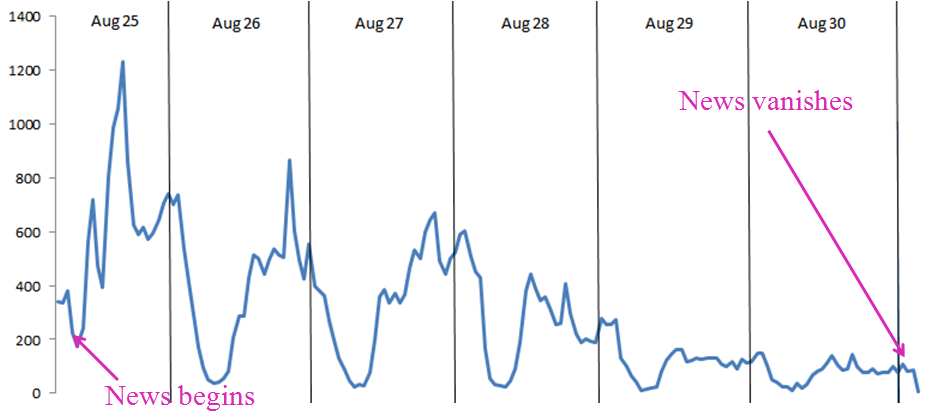
\includegraphics[width=3in,height=1.8in] {pictures/volume1.png}
\label{fig:Volume1}
}
\subfigure[Castro rumor]{
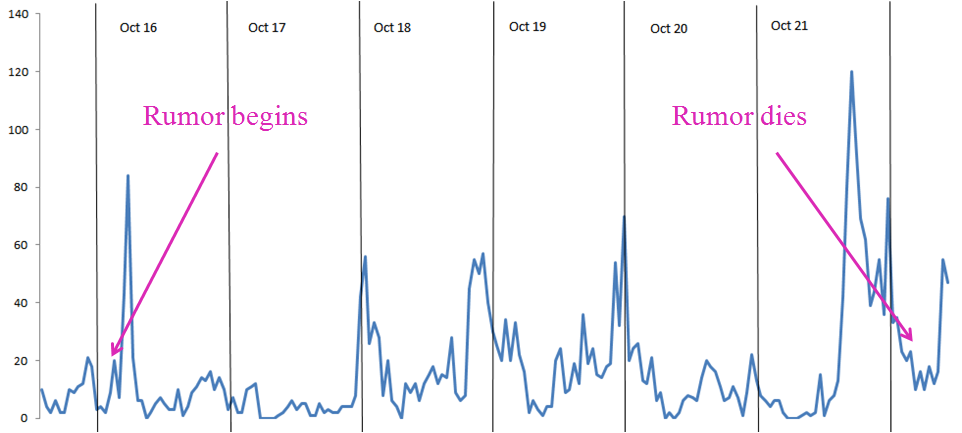
\includegraphics[width=3in,height=1.8in] {pictures/volume2.png}
\label{fig:Volume2}
}
\vspace{-1em}
\caption{Tweet volume.}
\label{fig:Volume}
\end{figure}

\subsection{Rumors}

\noindent
\textbf{\emph{Obama injured.}}
A fake associated press (AP) tweet originated on April 23, 2013 that President
Obama was hurt in White House explosions which caused a brief period of
instability in financial markets. The information was false
and it was determined that the Twitter account was hacked.

\noindent
\textbf{\emph{Doomsday.}}
December 21, 2012 was rumored to be the Doomsday as it marked the end date of a 5126 year long cycle in the Mesoamerican long count calendar. This rumor
spread like wildfire and social networks were flooded with panic and anxiety posts. Considering that we are still alive, Doomsday turned out to
be nothing more than a rumor on a massive scale\footnote{http://en.wikipedia.org/wiki/Doomsday}.

\noindent
\textbf{\emph{Fidel Castro's death.}}
On October 16, 2012 a Naples doctor claimed that former Cuban leader, Fidel Castro suffered a cerebral hemorrhage and is near a
neurovegetative state. However, on October 21, 2012, these rumors were denied
by Elias Jauva, former Venezuelan vice president, who released pictures of him
meeting Castro a few days back\footnote{http://www.inquisitr.com/371007/fidel-castro-allegedly-appears-in-public-after-stroke-rumors/}.

\noindent
\textbf{\emph{Riots and shooting in Mexico.}}
A very interesting example that highlights the perils of rumor spreading on social networks pertains to the false reports of violence and impending attack
in Nezahualcoyotl, %\narenc{Is it the correct spelling? Please checkup carefully. correct}
Mexico. (False) rumors spreading on Twitter and Facebook
about shootouts caused (real) panic and chaos in Mexico City
on September 5, 2012. Interestingly, authorities themselves
turned to Twitter to deny
these rumors\footnote{http://www.foxnews.com/world/2012/09/08/tweets-false-shootouts-cause-panic-in-mexico-city/}.



\begin{figure}[t]
\centering
\subfigure[Amuay explosion]{
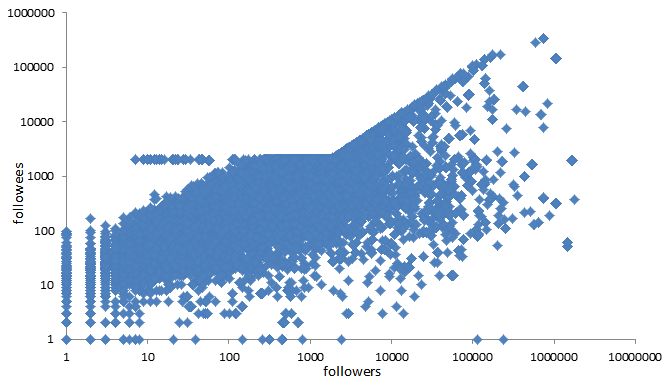
\includegraphics[width=3in,height=1.8in] {pictures/rumor1-scatter.png}
\label{fig:Follow1}
}
\subfigure[Castro rumor]{
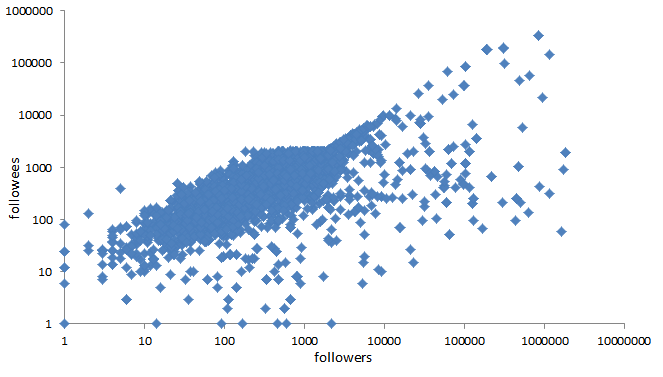
\includegraphics[width=3in,height=1.8in] {pictures/rumor2-scatter.png}
\label{fig:Follow2}
}
\vspace{-1em}
\caption{Followers/followees distributions. Followers: people who follow the person; Followees: people who are followed by the person.}
\label{fig:Followers}
\end{figure}
%\footnote{http://confusedofcalcutta.com/2009/01/11/of-followers-and-followees-and-friends/}

%\subsection{Twitter news collection }
%During data collection from Twitter, our main concern was to obtain pure tweets which are highly related to the news events. We used a customized set of keyword lists and hashtags for filtering the tweets. For each story, we created topic-exclusive keyword list and filtered the relevant tweets by matching the keywords. More story-specific tweets were identified by using a list of $\#$hashtags.
%
%As our stories span across geographic locations and languages, we used several different measures to collect the data. For example, four out of the eight stories are from South America, and hence during data collection for these stories we restricted ourselves to the tweets originating from South America and written either in Spanish or Portuguese. Table 1 list out all the restrictions that were used in collecting the tweets. Further, for each of these topics, we tried to collect the tweets from the beginning of the topic birth to its death. The only exception is the Doomsday rumor for which there is not fixed beginning date. Date range for data collection, along with the keywords, hashtags and tweet counts are mentioned in Table~\ref{table:story-intro} for each of the news story.

\begin{figure*}[t]
\centering
\subfigure[Amuay Cascade]{
   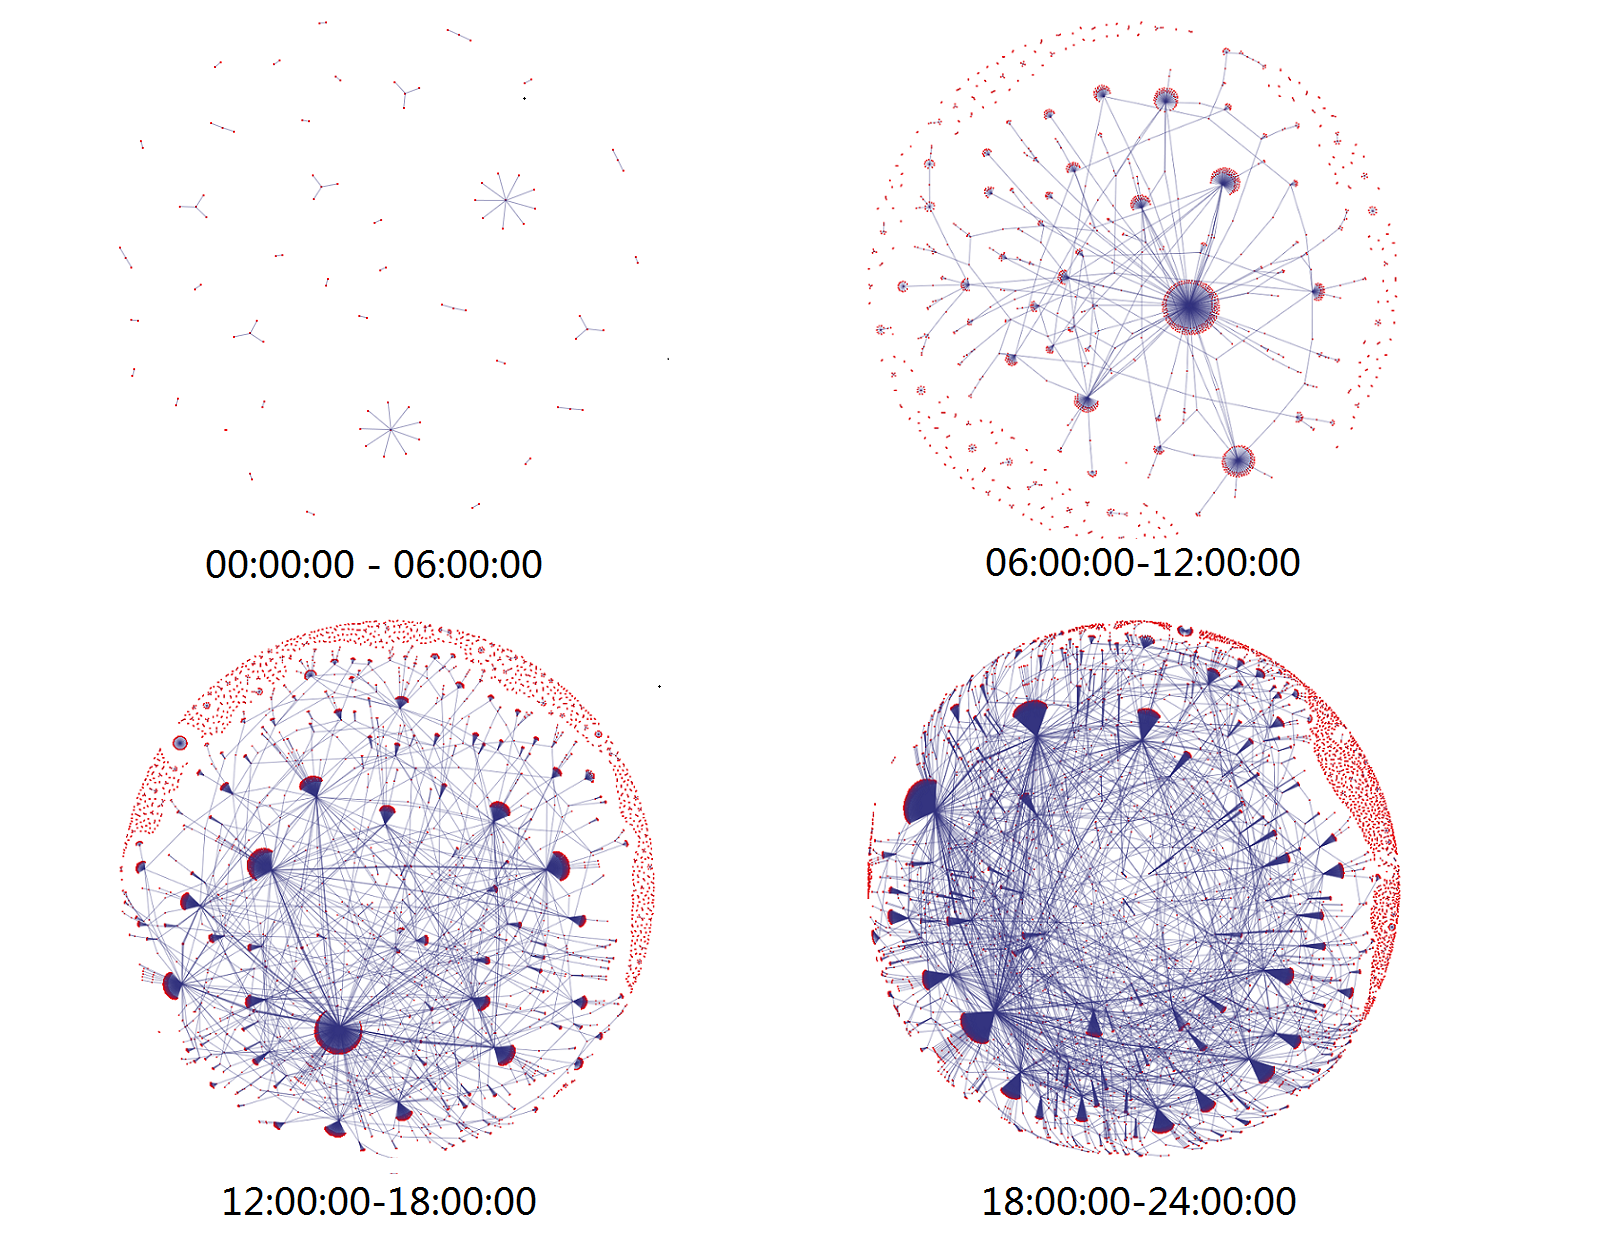
\includegraphics[width=3in,height=2.5in] {pictures/news.png}
   \label{fig:gas-cascade}
 }
  \subfigure[Castro Cascade]{
   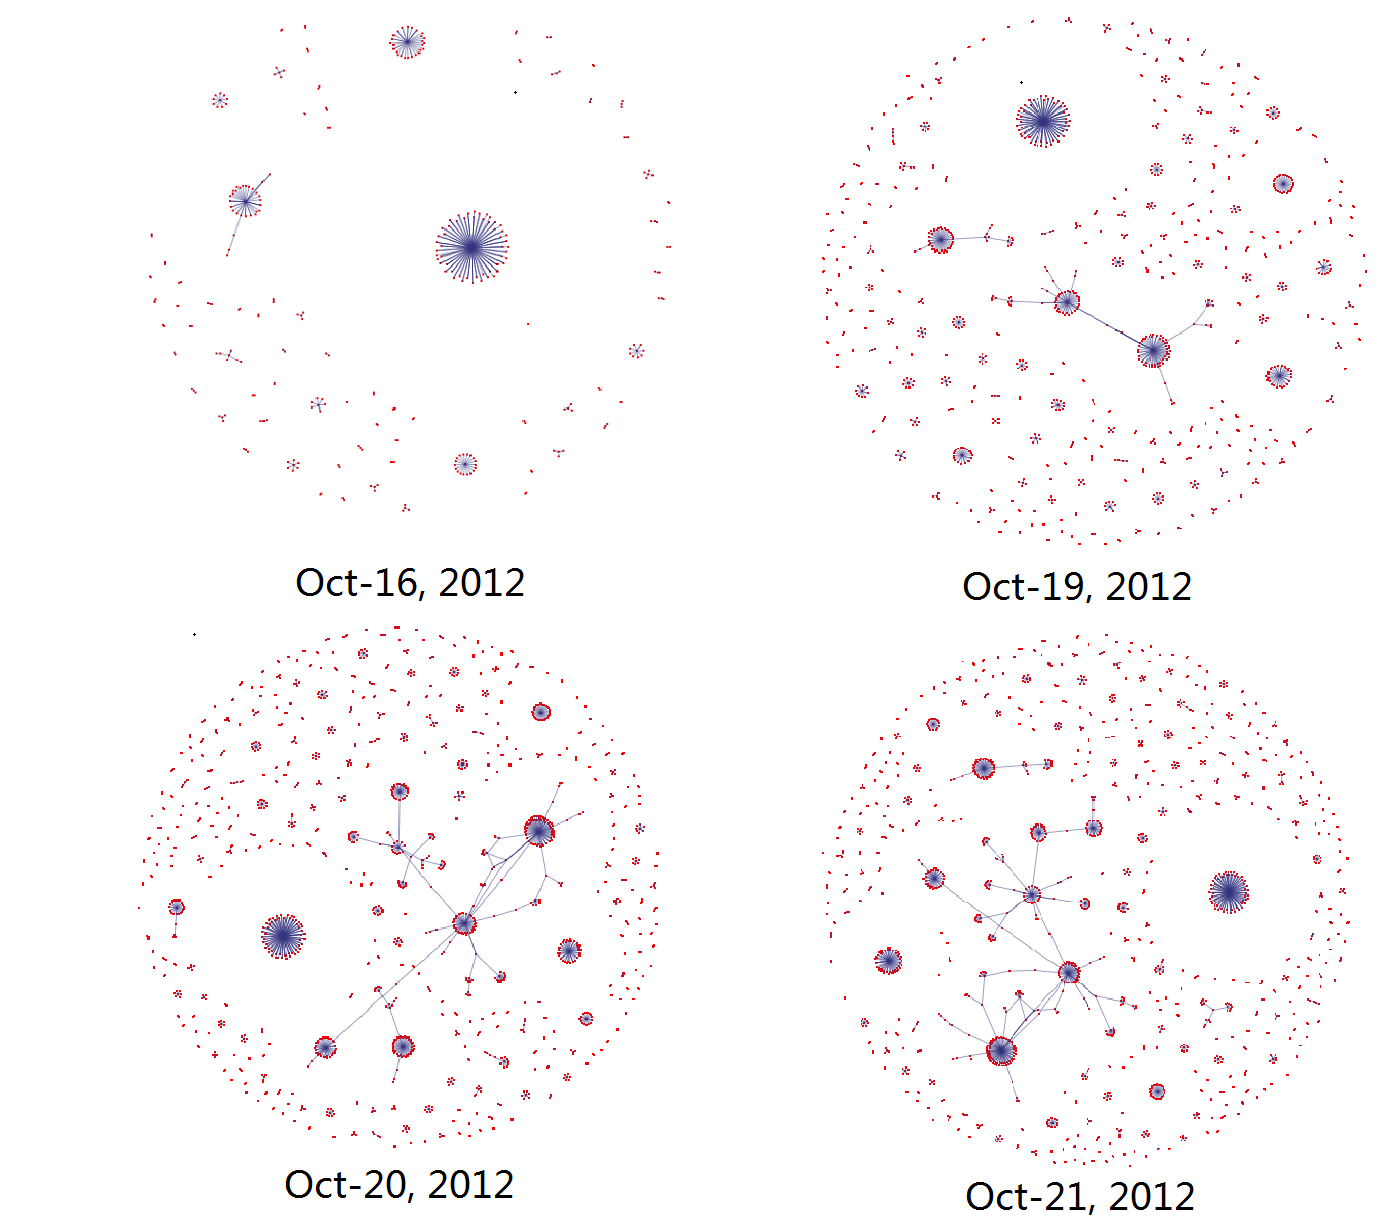
\includegraphics[width=3in,height=2.5in] {pictures/rumor.png}
   \label{fig:Castro-cascade}
 }

\caption{Retweet cascade for the Amuay Explosion news and Castro rumor. Each node is a user id, and each edge connects the retweet user to the original user.}
\label{fig:full-cascade}
\end{figure*}


\subsection{Preliminary Analysis}
We compare the basic properties of news and rumor propagation,
by characterizing
tweet volume over time, follower/followee distributions, the `response ratio'
of a story, and the retweet cascades. In order to maintain brevity, we show
results from only two stories in this section: one from our news
collection (the Amuay explosion) and one from our rumor collection (Fidel
Castro's purported death).

\textbf{Tweet Volume.} For both examples, we plot the tweet volume over time from the beginning of the story. Figure~\ref{fig:Volume1} shows the activity for the
2012 Amuay refinery explosion example. An activity burst was formed immediately after the news was made public. The number of tweets dropped progressively as the days went by. This activity trend displays attributes similar to breaking news propagation as described by Mendoza
et al.~\cite{Mendoza:2010}. In contrast, Figure~\ref{fig:Volume2} depicts
the volume of tweets about a rumor regarding the health of the
former Cuban leader Fidel Castro. Here we see
occasional spikes of
tweet volume; note the increase in tweet volume
around October 21st, when the rumors were officially denied.

\textbf{Followers and Followees Distributions.} Figure~\ref{fig:Follow1} is a log-log
scatter plot of the followers/followees distribution about
the Amuay explosion news, and Figure~\ref{fig:Follow2} is the corresponding
plot about Fidel Castro's death rumor. There is no significant
qualitative or quantitative difference in this case; in particular both
plots show that
the number of followees is less than the number of followers.
%Table~\ref{table:follower} gives the details: %in Amuay dataset, 33936 users
%%register more followers than followees (69\%),
%%14936 users register more followees than followers, and 143 users register
%%the same number of followers and followees.
%Amuay news and the Fidel Castro rumor exhibits comparable percentages for follower and followee.

%\begin{table}[ht]
%\centering
%\caption{Follower (ER) and followee (EE) distribution for two datasets.}
%\label{table:follower}
%\begin{tabular}{|c|c|c|l|} \hline
%&ER>EE&ER=EE&ER<EE\\ \hline
%Amuay news & 33936 (69\%)& 143 (1\%)&14936 (30\%)\\
%Castro rumor &2549 (66\%)& 13 (0.4\%)&1073 (33\%)\\ \hline
%\end{tabular}
%\end{table}

\textbf{Response Ratio.} A tweet can either be a post made by the
user's initiative,
or a responsive post  to some other user's post (e.g., retweets and replies).
As Starbird et al.~\cite{Starbird:2012} discuss, retweets reveal how
information propagates through a social network: the `deeper' a retweet, the
more relevant the tweet is for the community. Based on this idea,
we define the response ratio of a story as the fraction of responsive tweets
to the total number of tweets in the story.
Table~\ref{table:story-intro} lists the response ratio for all the 8 stories. As we can see, response ratios for news are higher than that for the rumors.
%\narenc{You keep using different names: response ratio, responsiveness ratio,
%response rate, responsiveness rate. Pick one and stick with it.
%Lets use response ratio because I don't think you are computing any `rate'.}
%\narenc{You have now removed that column from the table. Put it back.}

\textbf{Retweet Cascades.} A retweet cascade reflects how the social media network propagates information. Figure~\ref{fig:full-cascade} depicts the evolution of the retweet graphs for the Amuay news and Castro rumor dataset. For Amuay news, we plot four graphs with intervals of 6 hours,
% to show the dynamic process of the information flow on the Twitter.
depicting that a burst has been formed during 6am-12am, only 5 hours after the accident.
 %In the following hours, ten of thousands of users got this news from many sources.
 Fig.~\ref{fig:Castro-cascade} shows the retweet graphs of the rumor for several days. We can see
% that there are several central information sources to expand the rumor on Oct 16th, 2012.
 even after one day, there is no burst of tweets related to this rumor.
% After the clarification of the rumor, a little more users are involved in the re-tweet network.
 Compared with the network between the news and rumors, we find several features about the rumor.
% 1) In the initial  stage of the rumor, several central information sources posts the rumors.
1) The network for the news instance
is more complex and users can obtain news from many sources, while users obtain
the rumor information only from limited information centers. 2) There is an immediate burst after a news is made public while there is no obvious burst for the rumors.

%\narenc{What do people learn from this paragraph and the picture? Can you plot
%it for the Castro rumor? Does it look different?}

%\textbf{Can we learn more?} Although these properties provide us
%with some discriminating information, they still do not help
%develop a model-based approach for how news propagates differently
%from rumors, which is our focus next.

%with good amount of information we still can't quantify how news propagates over time. Also it would be interesting to know how information cascades were generated in a step by step manner over space. Hence, in this chapter, we propose a diffusion method and an event-driven model to find answers to the above mentioned problems. We represent Twitter network as a graph with vectors and edges and apply two epidemic models to simulate how vectors and edges grow with time. More specifically, we propose a 1-step graph transition method to simulate the graph growing process. By monitoring the step by step propagation process, we quantify transfer deviation using our event-driven model.
